%%%%%%%%%%%%%%%%%%%%%%%%%%%%%%%%%%%%%%%%%%%%%%%%%%%%%%%%%%%%
%%
%% WIKIPEDIA
%%
%%%%%%%%%%%%%%%%%%%%%%%%%%%%%%%%%%%%%%%%%%%%%%%%%%%%%%%%%%%%
\section{Wikipedia}
\label{sec:wikipedia}

%% Despite early skepticism (particularly concern over the inherent chaos
%% in the system: ``...edits, contributed in a predominantly undirected
%% and haphazard fashion by ... unvetted
%% volunteers.''\cite{Wilkinson2007}), Wikipedia is widely claimed to be
%% a great success, `the best-developed attempt thus far of the enduring
%% quest to gather all human knowledge in one
%% place'\cite{Mesgari2014}. The website is only around a decade old, but
%% in that time it has become a pre-eminent source of knowledge one the
%% internet. As a highly populous, visible and accessible online space,
%% the site is 

%% It is one of the most visited sites in the world, and the
%% most visited reference site by far. It is a huge site, with over 4.5
%% million article, in around 300 language languages, and is completely
%% open source and free-of-charge. It is an unparalleled data source,
%% detailed and easy to access.

%% However, one of the major factors contributing to the proliferation of
%% academic work on Wikipedia is suspicion. Investigations into the worth
%% and quality of Wikipedia articles abound. Work in this area ranged
%% from popular science to production software to full-blown academic
%% theses, and until around 2010 continued to be a well-visited topic.

%% In recent years, however, the research into Wikipedia's extrinsic
%% quality has waned. These studies peaked at around 2007, in the release
%% of the Wikitrust software, which brought together much of the
%% preceding research on the subject, and is discussed later. Since then,
%% though, papers on Wikipedian quality became less frequent, and
%% Wikipedia reached real omnipresence.  In these years, while the fears
%% that these crowd-sourced articles would supersede established
%% reference tomes were certainly realised, so did the public seem to
%% maintain a healthy suspicion of the site. Wikipedia is a central point
%% of fact-checking, with even search tools such as Google's voice search
%% and Apple's Siri taking it's content for granted, serving up
%% Wikipedian content automatically after voice searches, but the site is
%% still not accepted as a citable source.

%% Criticisms of Wikipedia still exists, however. Though, whilst they
%% began as investigations into external quality, now they more often
%% than not concern Wikiepdia's internal health. We can no longer argue
%% about whether or not the public should be reading these articles --
%% they already are. Instead, we examine the internals of Wikipedia, and
%% into the community that is involved in its growth. 

%% This is the context for our study. We can assume that an article has
%% worth, we don't care what that might be. We look at how this
%% may be distributed within the article. What can we find out about the
%% article by examining it's construction? What can we automatically
%% measure of a revision's text?

%% The objective of this project was to find a fair and concise way to
%% analyse a Wikipedia revision, both in terms of the text operations,
%% and in terms of an edits significance in the overall history of the
%% article.

Wikipedia is a free, open-source, publicly-editable online
knowledge-base. The software is runs upon, the PHP-based MediaWiki, is
also open-source, powering countless other online encyclopedias. The
website is ranked 6\super{th} globally in terms of website traffic,
and is the highest-ranked reference website by far - most of the sites
it shares the top spots with are commercial portals, search engines,
shopping mega-sites, and social media websites.\footnote{According to
  `Alexa', an website ranking company.\cite{Alexa-about2014} Though,
  this may be an underestimation. Alexa may well be biased towards
  English speakers and Internet Explorer users, underestimating
  Wikipedia.org's popularity, since `two thirds of all Wikipedia
  articles are in languages other than
  English'\cite{wikimedia-noteonalexa}}\label{sec:popularity} Despite
early skepticism (particularly concern over the inherent chaos in the
system: ``...edits, contributed in a predominantly undirected and
haphazard fashion by ... unvetted volunteers.''\cite{Wilkinson2007}),
it is widely claimed to be a success, `the best-developed attempt thus
far of the enduring quest to gather all human knowledge in one
place'\cite{Mesgari2014}.

That Wikipedia has become a hub of research in many fields is also
self-evident to anyone who has searched for articles on the
subject. Mesgari et al, just quoted, has prepared a very recent
`systematic review of scholarly research on the content of Wikipedia',
which gives an overview of 110 articles on the subject --- attesting
to his observation that Wikipedia has been `irresistible point of
inquiry for researchers from various fields of knowledge'. It will be
a useful touching stone for this study, finding 82 out of the 110
surveyed articles to concern Wikipedia quality. Some of these are also
referenced here.

Other important general sources have been WikiLit,\cite{wikilit}
AcaWiki\cite{acawiki} and WikiPapers\cite{wikipapers}, all of which
are online repositories of academic research into Wikipedia and other
Wikis, and from which many of the studies mentioned here were found.

%%%%%%%%%%%%%%%%%%%%%%%%%%%%%%%%%%%%%%%%%%%%%%%%%%%%%%%%%%%%
%%
%% WIKIPEDIA ARTICLE QUALITY
%%
%%%%%%%%%%%%%%%%%%%%%%%%%%%%%%%%%%%%%%%%%%%%%%%%%%%%%%%%%%%%

\subsection*{Existing studies of Wikipedia revision history}
Tangentially related studies fall into two major groups: studies of
Wikipedia article quality and studies of edit behaviour.  It is from
the first group that we find the most pertinent work --- it is also
one of the most fruitful areas of research.

It is the metrics used to measure quality in these studies that are of
most use to us here. We don't concern ourselves with the external
quality rather how successful the article is in its own context of
Wikipedia, but many studies have endeavoured to find out what kind of
article content can be automatically recognised. We can also assume
that editors may well appraise an article in a similar way to the
passive, Wikipedia-innocent reader-agents these studies concern
themselves with.

High numbers of Links, internal links, images and formulas have been
found to indicate perceived
quality,\cite{Lucassen2010}\cite{mcguinness2006} and these are easy to
identify using Wikipedia's markup language. Other useful metrics have
been the age of the word,\cite{Cross2006} the age and rate of change
of the article in comparison to other articles,\cite{Zeng2006} and the
recent activity of the article (an article undergoing a peak in edit
changes may be `unstable').\cite{Adler2006} Another study of
particular interest is that of Stvilia et al, which found metrics of
article quality through factor analysis,\cite{Stvilia2005} confirming
much of the ideas already mentioned. A particularly interesting study
found simply that word count maps well to success within Wikipedia,
with longer articles receiving `featured article'
status.\cite{blumenstock2008size}

A landmark piece of work is the Wikitrust software.\cite{Adler2007}
Wikitrust was\footnote{Defunct as of author's checks, Apr 2014} a
firefox plugin, designed to highlight the words of a Wikipedia article
with different colors, building upon the writing of Cross,
2006.\cite{Cross2006} The gradations of these colors relate to levels
of `trust', and in turn on both the word's age, and the trust rating
of the editor that contributed that word. A screenshot can be seen in
figure \ref{fig:wikitrust}. 

The program was reviewed as recently as 2011,\cite{Lucassen2011} and
it was found to be basically flawed, with users not really seeing the
use for it. In fact, as a foil to the `na\"ive reader' paradigm
assumed by many of these studies, it was found that, having used
Wikipedia before, readers already had personal methods for deciding
whether to trust of not trust a Wikipedia article. 

\begin{figure}
  \centering
  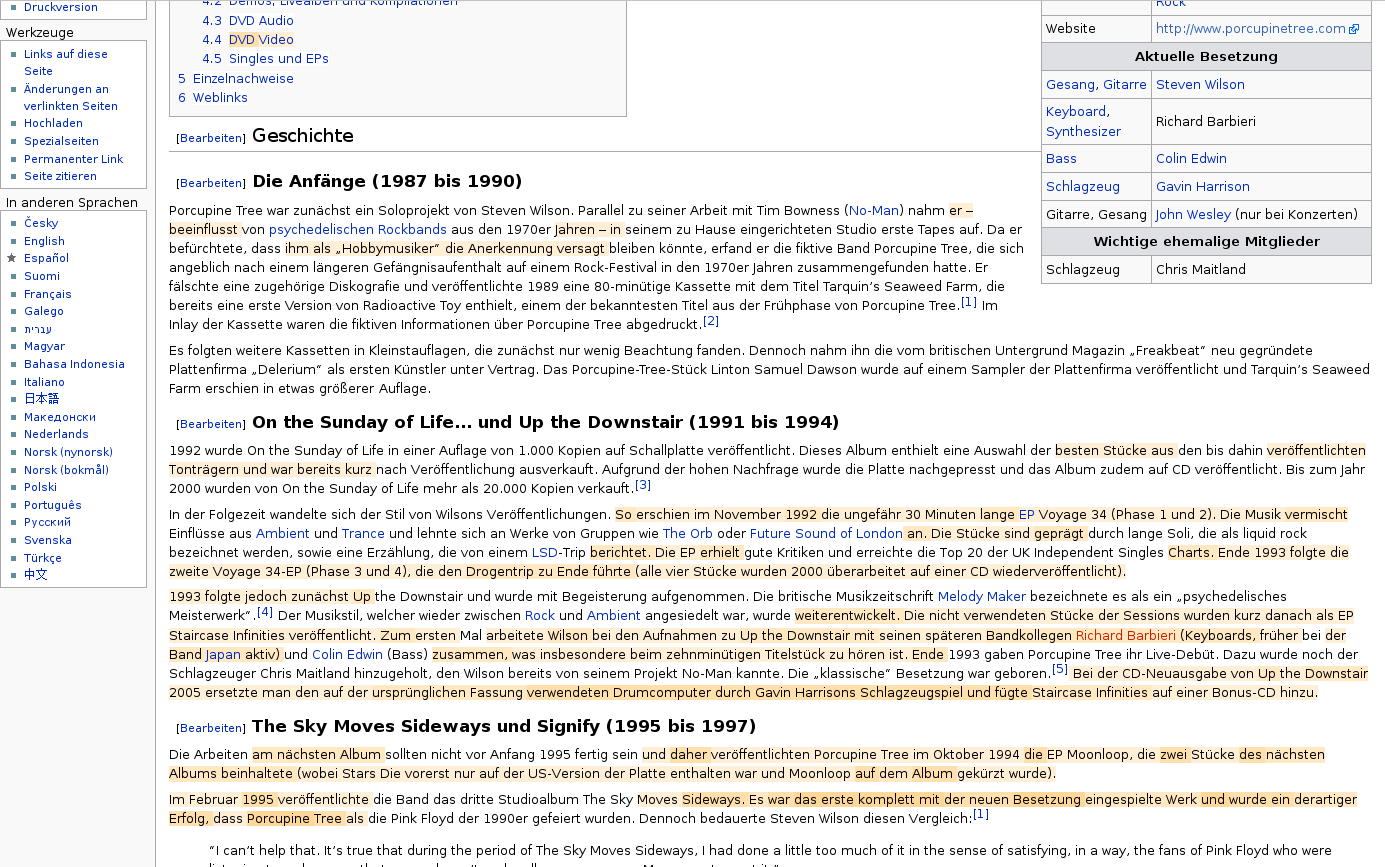
\includegraphics[width=0.8\textwidth,clip=true,resolution=300]{img/wikitrust.png}
  \caption{Wikitrust in action, 2011}
  \label{fig:wikitrust}
\end{figure}

A few other studies present us with useful analyses of edit
behaviour. These studies turn to Wikipedia in order to study user
network interaction, and these analyses of conflict between editors
show the possible reversion cases we will have to automatically
recognise. 

They reveal the high number of immediate `undo'-type revisions, and
also that malicious or unnecessary input may survive several versions
before being undone. Some study these conflicts as a characterisation
of normal editing
behaviour,\cite{Kittur2007}\cite{Kittur2009}\cite{Kittur2010}\cite{Potthast2008}
while others look to controversial articles,\cite{Iba2010} or articles
recently cited in the press.\cite{Lih2004} We find from these same
studies that articles lead by small groups of `leaders' produce
articles of better quality than those with a more homogeneous
contribution group, that a small group of editors contribute to most
of Wikipedia, and that conflict and bureaucracy (increasing over time)
are the major limiting factors in the growth of an
article.\cite{Suh2009} 
